\chapter{Principles and Components of Sensor Fusion Systems}
\label{sec:Principles}
%
%
% ============================================
%\textcolor{red}{[GAB: can we break this section in at least a couple of subsections? otherwise the Table of contents looks too empty for this section.]}

%[I do not see a way to break this section in a nice way and keep the good flow. I suggest we do not bother breaking it]


% Springer Nature: each chapter should have a 10--15 line online abstract.
% This chapter abstract has not yet been written in the uploaded manuscript.
\abstract{\added{This chapter describes the components and the system-level requirements that any sensor fusion system must satisfy, independently of the particular mathematical tools chosen to combine the data. A generic pipeline is introduced, from data acquisition through preprocessing, representation and fusion to inference and application, together with the feedback loops through which fused outputs adapt models, sensor weights and calibration. The level at which fusion takes place, from raw data through features and objects to decisions, is tied to the choice of representation, which ranges from raw signals, feature vectors and tracks to occupancy grids, belief distributions, bounded sets and learned embeddings. Representative application areas, from autonomous vehicles, drones and robots to smart infrastructure, industrial automation, healthcare, extended reality and remote sensing, are surveyed to show that fusion is a cross-domain design pattern whose common requirements are heterogeneity, uncertainty, operational constraints and robustness. The main building blocks of a fusion system are then summarised: sensing sources, temporal and spatial alignment, representation and abstraction level, uncertainty and reliability modelling, the fusion mechanism, inference and downstream use, and adaptation and validation. The chapter closes by characterising the outputs of a fusion system, which are never a bare point estimate but always an estimate accompanied by a covariance, a bounded set, an existence confidence or a conflict indicator, and by motivating the classical methods reviewed next.}}
\suppressfloats[t]

Sensor fusion systems are organised around the principle that heterogeneous observations can be transformed into a common, uncertainty-aware representation that is more informative than any individual source alone. In practice, this requires more than simply combining measurements. A complete fusion system must acquire data from different sensors, compensate for sensor-specific errors, align measurements in time and space, choose an appropriate representation, apply a fusion rule or learning architecture, and deliver outputs that can be used by downstream inference, planning, control, or decision-making modules \cite{hall_introduction_1997,luo_multisensor_1989,liggins_handbook_2009,khaleghi_multisensor_2013}. These components form the conceptual bridge between the general motivation introduced above and the specific classical and learning-based methods reviewed in the following sections.

\begin{figure}[!t]
    \centering
    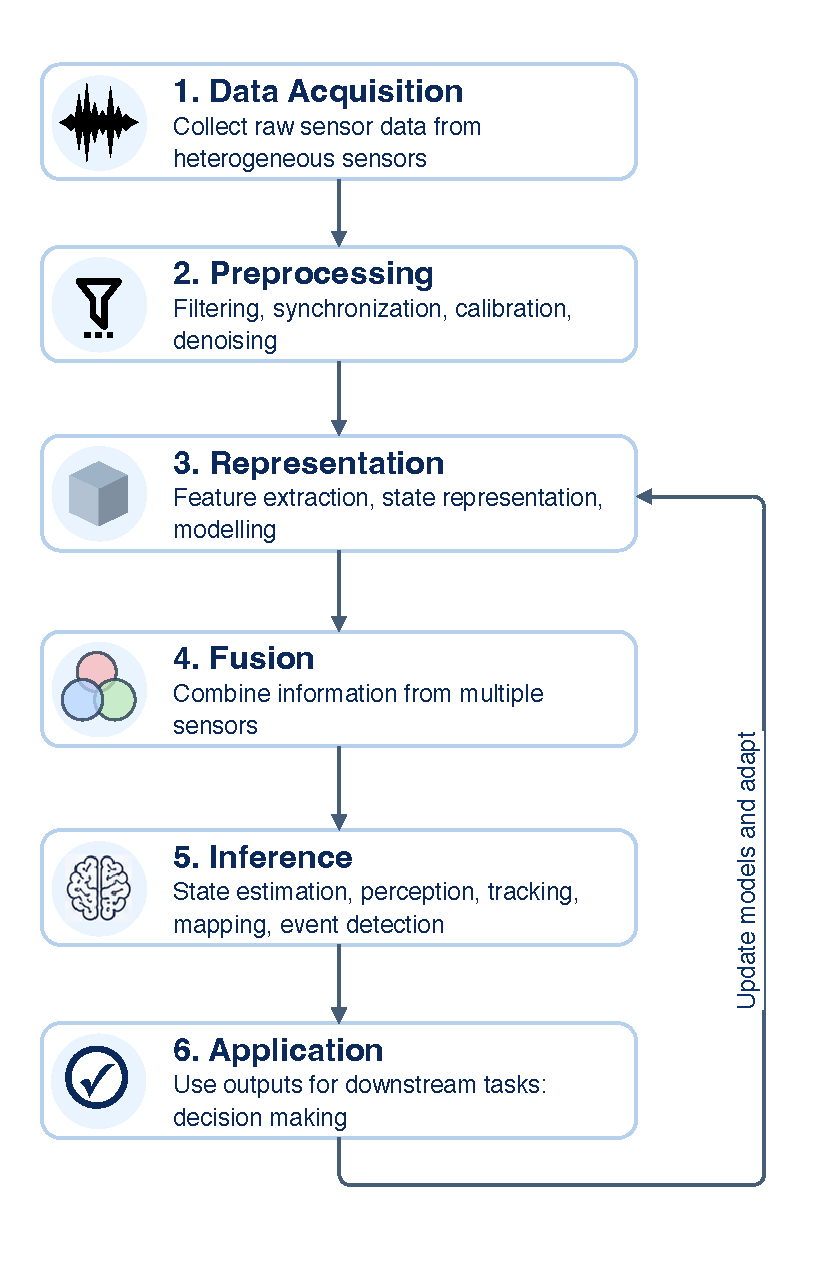
\includegraphics[width=0.85\columnwidth]{figures/fusion_pipeline_v02.pdf}
    \caption{A typical sensor fusion pipeline, from heterogeneous data acquisition to downstream application and feedback-based adaptation.}
    \label{fig:generic-sensor-fusion-pipeline}
\end{figure}

Figure~\ref{fig:generic-sensor-fusion-pipeline} summarises a generic fusion pipeline. The first stage is \emph{data acquisition}, where raw observations are collected from heterogeneous sensors or information sources. These measurements may differ in physical modality, sampling frequency, dimensionality, noise statistics, field of view, latency, and failure modes. The second stage is \emph{preprocessing}, which includes filtering, synchronisation, calibration, denoising, outlier rejection, missing-data handling, and coordinate-frame alignment. This stage is essential because fusion algorithms generally assume that measurements refer to compatible physical quantities, time instants, or spatial frames.

The third stage is \emph{representation}. Depending on the application, sensor measurements may be represented as raw signals, feature vectors, tracks, point clouds, occupancy grids, semantic objects, belief distributions, sets, or learned latent embeddings. The choice of representation strongly affects the level at which fusion is performed. Data-level fusion combines low-level measurements directly; feature-level fusion combines extracted attributes or learned representations; object-level fusion combines detections, tracks, or state estimates; and decision-level fusion combines classifier outputs, alarms, or symbolic decisions. The fourth stage is the actual \emph{fusion} step, in which information from multiple sources is combined using statistical estimation, Bayesian filtering, evidence theory, optimisation, set-membership methods, fuzzy reasoning, machine learning, or hybrid approaches.

The final stages convert fused information into task-relevant knowledge. The \emph{inference} stage estimates states, detects events, tracks objects, maps environments, classifies situations, or predicts future behaviour. The \emph{application} stage then uses these outputs to support downstream tasks such as monitoring, decision-making, planning, control, diagnosis, or human assistance. The feedback arrow in Fig.~\ref{fig:generic-sensor-fusion-pipeline} highlights that practical fusion systems are rarely one-pass pipelines: outputs can be used to update models, adapt sensor weights, refine calibration, select active sensing actions, or reconfigure the system when operating conditions change.

\begin{figure}[!t]
    \centering
    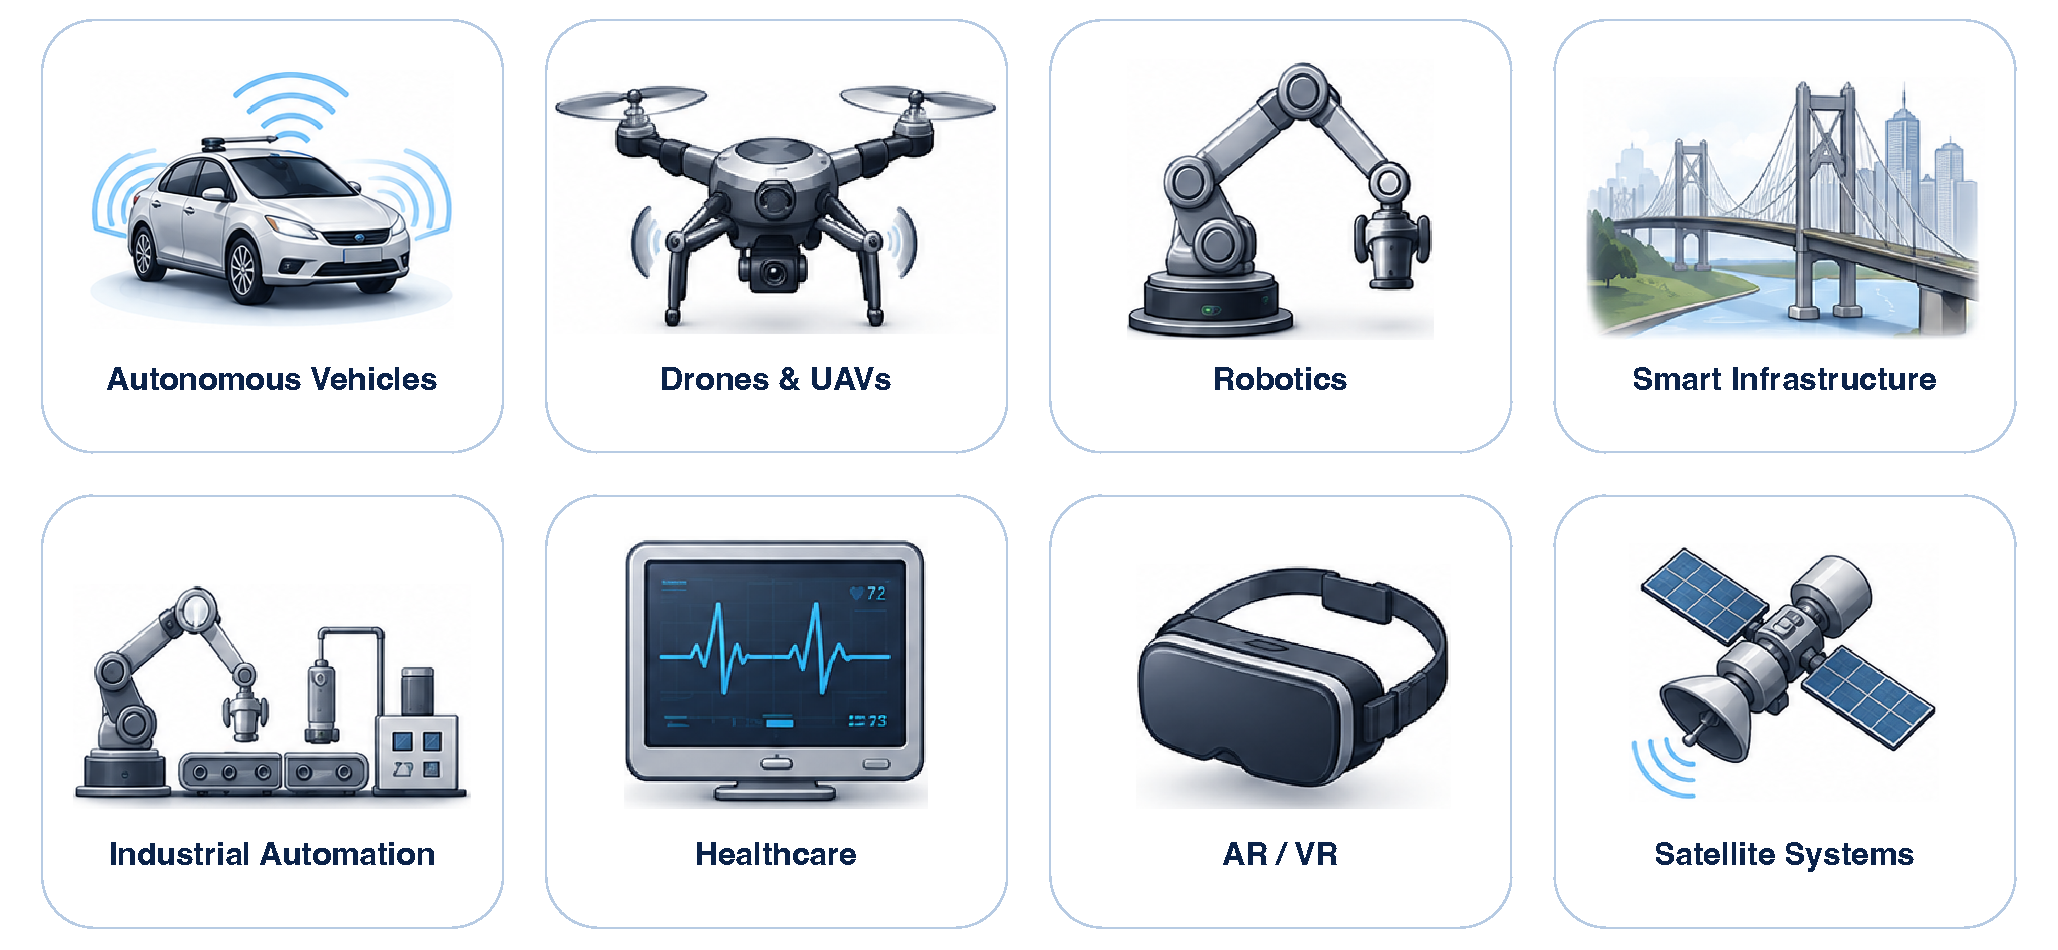
\includegraphics[width=1\columnwidth]{figures/application_areas.pdf}
    \caption{Representative application areas of sensor fusion.}
    \label{fig:application-areas}
\end{figure}

As illustrated in Fig.~\ref{fig:application-areas}, sensor fusion is a cross-domain design pattern rather than a technique restricted to a single field. Autonomous vehicles integrate cameras, radar, LiDAR, inertial sensors, positioning systems, and maps to perceive dynamic road scenes and estimate ego-motion. Drones and unmanned aerial vehicles combine inertial, visual, GNSS, barometric, and range measurements for navigation, stabilisation, obstacle avoidance, and mapping. Robotic systems fuse proprioceptive and exteroceptive sensing to support localisation, manipulation, force control, human--robot interaction, and task planning.

Smart infrastructure combines distributed structural, environmental, traffic, and communication data to monitor bridges, roads, buildings, and energy systems. Industrial automation uses fusion to improve quality control, predictive maintenance, process monitoring, and safe collaboration between humans and machines. Healthcare systems combine physiological, imaging, wearable, and contextual data for diagnosis, monitoring, rehabilitation, and decision support. AR/VR systems fuse cameras, IMUs, depth sensors, eye tracking, and environmental maps to provide robust pose estimation and spatial interaction. Satellite and remote-sensing systems combine optical, radar, thermal, multispectral, and communication data to observe large-scale environmental and human activity.

Although these domains differ substantially, they share a common set of system-level requirements. First, fusion must address \emph{heterogeneity}: the input data may describe appearance, geometry, motion, range, force, acceleration, temperature, physiology, or communication events. Second, fusion must handle \emph{uncertainty}: measurements may be noisy, ambiguous, delayed, intermittent, biased, or contradictory. Third, fusion must satisfy \emph{operational constraints}: many applications require real-time or near-real-time performance on embedded or distributed hardware. Fourth, fusion must support \emph{robustness}: safety-critical systems must continue operating under sensor degradation, environmental changes, communication losses, and out-of-distribution conditions. These requirements explain why the field contains both model-based methods, which provide explicit uncertainty handling and interpretability, and learning-based methods, which provide rich representations for complex multimodal data.

From a design perspective, the main components of a sensor fusion system can therefore be summarised as follows:
\begin{list4a}
    \item \textbf{Sensing sources}: physical sensors, virtual sensors, maps, communication messages, historical data, and model predictions that provide partial information about the system or environment.
    \item \textbf{Temporal and spatial alignment}: synchronisation, interpolation, latency compensation, intrinsic calibration, extrinsic calibration, and coordinate transformations that make heterogeneous data comparable.
    \item \textbf{Representation and abstraction level}: raw measurements, engineered features, learned embeddings, detections, tracks, occupancy maps, semantic maps, probability distributions, bounded sets, or decisions.
    \item \textbf{Uncertainty and reliability modelling}: probabilistic noise models, confidence scores, belief masses, fuzzy memberships, deterministic bounds, sensor-health indicators, and context-dependent reliability weights.
    \item \textbf{Fusion mechanism}: algorithms or architectures that combine information, resolve conflicts, exploit complementarity, handle redundancy, and propagate uncertainty to later stages.
    \item \textbf{Inference and downstream use}: state estimation, perception, tracking, mapping, event detection, prediction, planning, control, monitoring, diagnosis, or decision support.
    \item \textbf{Adaptation and validation}: mechanisms for online model update, failure detection, recalibration, robustness assessment, uncertainty calibration, and verification under representative and rare operating conditions.
\end{list4a}

This system-level view motivates the organisation of the rest of the book. Chapter~\ref{sec:classicalSF} first reviews classical fusion techniques, including probabilistic, statistical, evidence-theoretic, optimisation-based, and set-membership approaches. Chapter~\ref{sec:learning} then examines learning-based and hybrid techniques, where multimodal representations are learned directly from data and combined with model-based estimation or decision-making. Throughout the book, autonomous driving is used as a concrete reference domain, while the underlying principles remain applicable to the broader application areas shown in Fig.~\ref{fig:application-areas}.

\begin{figure}[!t]
    \centering
    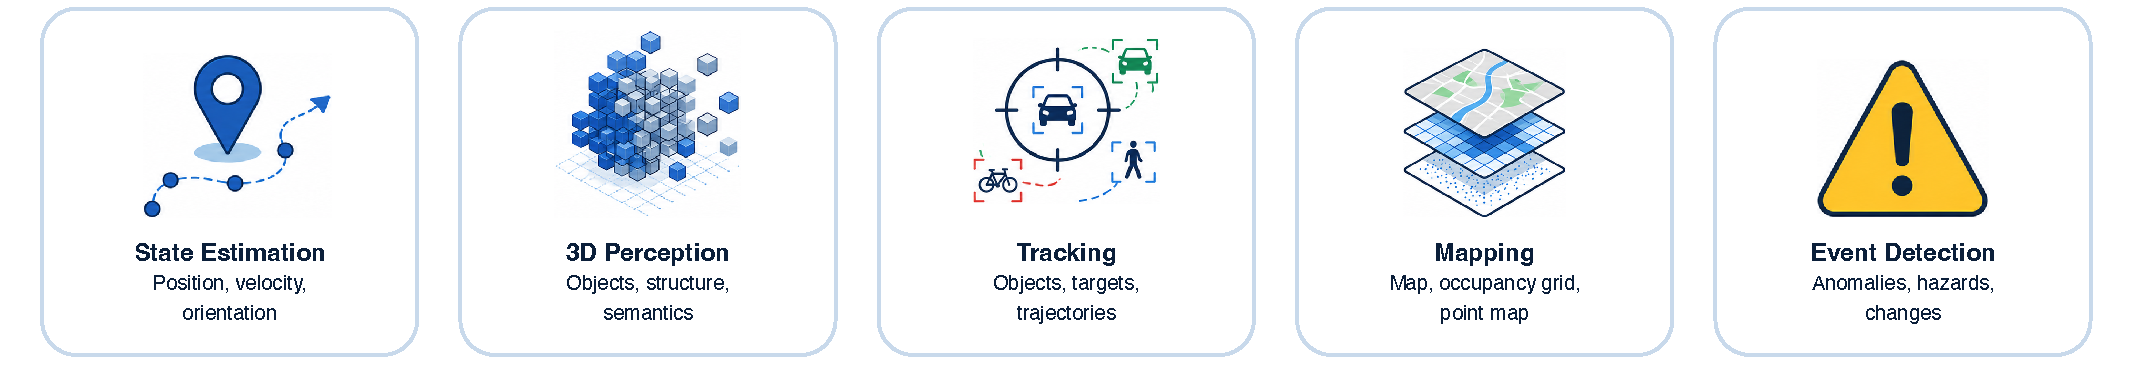
\includegraphics[width=1\columnwidth]{figures/estimates_outputs.pdf}
    \caption{Representative outputs produced by sensor-fusion systems, ranging from state estimates and tracks to maps, decisions, and uncertainty-aware alerts.}
    \label{fig:estimates-outputs}
\end{figure}

Figure~\ref{fig:estimates-outputs} emphasises that the output of a fusion system is not limited to a single point estimate. Depending on the application and abstraction level, fusion may produce filtered state estimates, covariance matrices, bounded state sets, object tracks, occupancy maps, semantic labels, anomaly scores, conflict indicators, reliability weights, or control-relevant decisions. These outputs should be interpreted together with their uncertainty and validity assumptions. For example, a vehicle pose estimate is useful only when accompanied by a covariance, confidence interval, or bounded error envelope; an object detection becomes more valuable when associated with a track identity and existence confidence; and a decision-level alert is safer when it exposes whether sensors agree, disagree, or are degraded. This motivates the transition from system components to the classical mathematical tools reviewed in the next section.

\begin{addedblock}
The component view of this chapter is also the key to the end-of-chapter problems of the following chapters. Each problem isolates one component of the pipeline, such as the weighting of two sources of different accuracy, the alignment of a delayed track, the propagation of a bounded set, or the resolution of a conflict between two classifiers, and asks the reader to carry out the corresponding computation by hand or with the companion repository. Reading a problem, it is therefore useful to ask first which block of Fig.~\ref{fig:generic-sensor-fusion-pipeline} it exercises and which of the outputs of Fig.~\ref{fig:estimates-outputs} it produces. The solutions collected at the end of the book return to this question explicitly whenever a numerical result has a system-level interpretation.
\end{addedblock}

% ============================================
%
%
